\begin{figure}[!htbp]
\centering
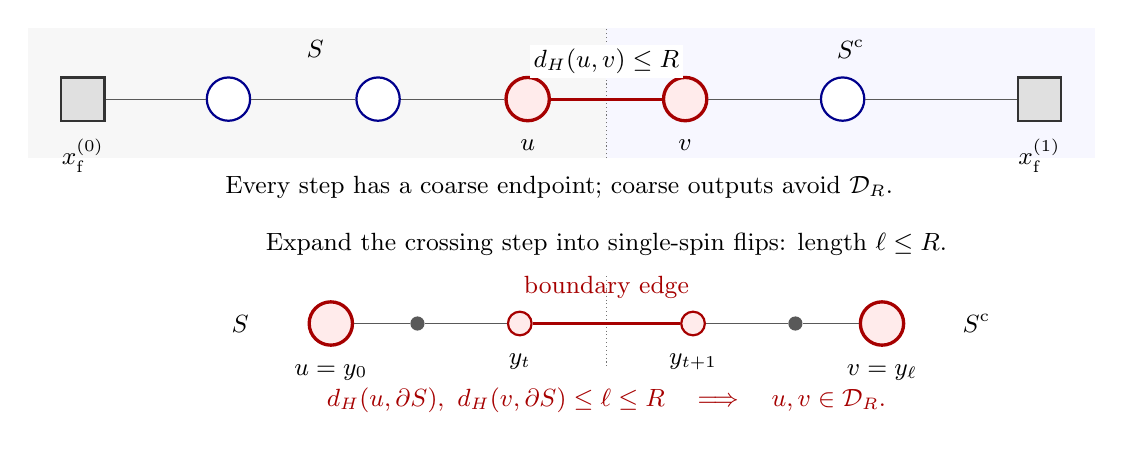
\begin{tikzpicture}[
  x=1cm,y=1cm,font=\small,
  coarse/.style={circle,draw=blue!55!black,fill=white,
    line width=.8pt,minimum size=5.5mm,inner sep=0pt},
  fine/.style={rectangle,draw=black!80,fill=black!12,
    line width=.8pt,minimum size=5.5mm,inner sep=0pt},
  forced/.style={coarse,draw=red!65!black,fill=red!8,line width=1.2pt},
  flip/.style={circle,fill=black!65,minimum size=1.8mm,inner sep=0pt},
  boundary/.style={circle,draw=red!65!black,fill=red!8,
    line width=.8pt,minimum size=3mm,inner sep=0pt}
]
  \fill[black!3] (-.05,-.75) rectangle (7.3,.9);
  \fill[blue!3] (7.3,-.75) rectangle (13.5,.9);
  \draw[densely dotted,black!55] (7.3,-.75) -- (7.3,.9);
  \node at (3.6,.63) {$S$};
  \node at (10.4,.63) {$S^{\mathrm c}$};

  \node[fine] (leftfine) at (.65,0) {};
  \node[coarse] (coarsezero) at (2.5,0) {};
  \node[coarse] (coarseone) at (4.4,0) {};
  \node[forced] (crossleft) at (6.3,0) {};
  \node[forced] (crossright) at (8.3,0) {};
  \node[coarse] (coarselast) at (10.3,0) {};
  \node[fine] (rightfine) at (12.8,0) {};
  \draw[black!65] (leftfine) -- (coarsezero)
    (coarsezero) -- (coarseone) (coarseone) -- (crossleft)
    (crossright) -- (coarselast) (coarselast) -- (rightfine);
  \draw[red!65!black,line width=1.1pt] (crossleft) -- (crossright);
  \node[below=1mm] at (leftfine.south) {$x_{\rm f}^{(0)}$};
  \node[below=1mm] at (rightfine.south) {$x_{\rm f}^{(1)}$};
  \node[below=1mm] at (crossleft.south) {$u$};
  \node[below=1mm] at (crossright.south) {$v$};
  \node[fill=white,inner sep=1.5pt] at (7.3,.48)
    {$d_H(u,v)\le R$};
  \node at (6.7,-1.12)
    {Every step has a coarse endpoint; coarse outputs avoid $\mathcal D_R$.};

  \node at (7.3,-1.85)
    {Expand the crossing step into single-spin flips: length $\ell\le R$.};
  \draw[densely dotted,black!55] (7.3,-2.25) -- (7.3,-3.4);
  \node[forced] (pathleft) at (3.8,-2.85) {};
  \node[flip] (pathone) at (4.9,-2.85) {};
  \node[boundary] (boundaryleft) at (6.2,-2.85) {};
  \node[boundary] (boundaryright) at (8.4,-2.85) {};
  \node[flip] (pathlast) at (9.7,-2.85) {};
  \node[forced] (pathright) at (10.8,-2.85) {};
  \draw[black!65] (pathleft) -- (pathone) (pathone) -- (boundaryleft)
    (boundaryright) -- (pathlast) (pathlast) -- (pathright);
  \draw[red!65!black,line width=1.1pt] (boundaryleft) -- (boundaryright);
  \node[above=2mm,red!65!black] at (7.3,-2.85) {boundary edge};
  \node[below=1mm] at (pathleft.south) {$u=y_0$};
  \node[below=1mm] at (boundaryleft.south) {$y_t$};
  \node[below=1mm] at (boundaryright.south) {$y_{t+1}$};
  \node[below=1mm] at (pathright.south) {$v=y_\ell$};
  \node at (2.65,-2.85) {$S$};
  \node at (12,-2.85) {$S^{\mathrm c}$};
  \node[red!65!black] at (7.3,-3.83)
    {$d_H(u,\partial S),\ d_H(v,\partial S)\le\ell\le R
      \quad\Longrightarrow\quad u,v\in\mathcal D_R$.};
\end{tikzpicture}
\caption{The boundary obstruction for the finite sequence of proposals.
In the upper chain, squares are fine endpoints and circles are coarse outputs; consecutive
configurations have Hamming distance at most $R$. When the fine endpoints lie on opposite sides, some consecutive pair
$u,v$ crosses the cut and contains a coarse output. A shortest path of
one-spin flips between that pair meets the two-sided boundary $\partial S$.
Its length is at most $R$, so both $u,v$ lie in
$\mathcal D_R=\{x:d_H(x,\partial S)\le R\}$, contradicting avoidance by
the coarse outputs. All geometry is schematic: grid outputs are
correlated, and lines do not represent continuous spin trajectories.}
\label{fig:connection}
\end{figure}
